\documentclass[11pt, addpoints, answers]{exam}

\usepackage{amsmath, amssymb}
\usepackage{xcolor}

\newcommand{\red}[1]{\textcolor{red}{#1}}

% For inserting code snippets.
\usepackage{listings}
\lstset{
    columns = fixed,
    basewidth = {0.5em},
    breaklines = true,
    backgroundcolor = \color{white},
    keywordstyle = \color[RGB]{40, 40, 255},
    numberstyle = \footnotesize\color{darkgray},
    commentstyle = \ttfamily\color{violet},
    basicstyle = \ttfamily,
    stringstyle = \ttfamily\color[RGB]{128, 0, 0},
    showstringspaces = false,
    language = {[11]C++},
    escapechar = \@
}
\lstnewenvironment{cpp}[1][]{\lstset{language = {[11]C++}, #1}}{}

\usepackage{tikz}
\usepackage{tikz-qtree}
\usetikzlibrary{positioning}


% headers, footers, titles
\newcommand{\CourseName}{CS101 Algorithms and Data Structures}
\newcommand{\HomeworkNO}{Homework 10}
\newcommand{\DueDate}{Due date: December 24, 2023, at 23:59}

\pagestyle{headandfoot}
\runningheadrule
\runningheader{\CourseName}{\HomeworkNO}{\DueDate}
\runningfooter{}{\thepage}{}

\title{
	\CourseName\\
	Fall 2023\\
	\HomeworkNO
}
\author{}
\date{\DueDate}

% formats of questions, choices, points, etc.
\qformat{\bf\thequestion. (\totalpoints\ points) \thequestiontitle\hfill}
\pointname{'}
\CorrectChoiceEmphasis{\bf\color{blue}}
\SolutionEmphasis{\color{blue}}

% We frequently use this font.
\newcommand{\ttt}{\texttt}
\newcommand{\bluett}[1]{\textcolor{blue}{\ttt{#1}}}

\begin{document}

\maketitle

\begin{enumerate}
	\item Please write your solutions in English.
	\item Submit your solutions to gradescope.com.
	\item Set your FULL name to your Chinese name and your STUDENT ID correctly in Account Settings.
	\item If you want to submit a handwritten version, scan it clearly. \ttt{CamScanner} is recommended.
	\item When submitting, match your solutions to the problems correctly.
	\item No late submission will be accepted.
	\item Violations to any of the above may result in zero points.
\end{enumerate}

\begin{questions}

\newpage

\titledquestion{Multiple Choices}

Each question has \textbf{one or more} correct answer(s). Select all the correct answer(s). For each question, you will get 0 points if you select one or more wrong answers, but you will get 1 point if you select a non-empty subset of the correct answers.

Write your answers in the following table.

%%%%%%%%%%%%%%%%%%%%%%%%%%%%%%%%%%%%%%%%%%%%%%%%%%%%%%%%%%%%%%%%%%%%%%%%%%%
% Note: The `LaTeX' way to answer a multiple-choices question is to replace `\choice'
% with `\CorrectChoice', as what you did in the first question. However, there are still
% many students who would like to handwrite their homework. To make TA's work easier,
% you have to fill your selected choices in the table below, no matter whether you use 
% LaTeX or not.
%%%%%%%%%%%%%%%%%%%%%%%%%%%%%%%%%%%%%%%%%%%%%%%%%%%%%%%%%%%%%%%%%%%%%%%%%%%

\begin{table}[htbp]
    \centering
    \begin{tabular}{|p{2cm}|p{2cm}|p{2cm}|}
        \hline
        (a) & (b) & (c)                \\
        \hline
        %%%%%%%%%%%%%%%%%%%%%%%%%%%%%%%%%%%%%%%%%%%%%%%%%%%%%%%%%%
        % YOUR ANSWER HERE.
        ABD & ACD & ABC \vspace{0.4cm} \\
        %%%%%%%%%%%%%%%%%%%%%%%%%%%%%%%%%%%%%%%%%%%%%%%%%%%%%%%%%%
        \hline
    \end{tabular}
\end{table}

\begin{parts}

    \part[2] Which of the following statements about Dijkstra's algorithm is/are true?

    \begin{choices}
        \CorrectChoice Once a vertex is marked as visited, its distance will never be updated.
        \CorrectChoice The time complexity of Dijkstra's algorithm using complete binary heap is $\Theta(|E|\log |V|)$.
        \choice If we use Dijkstra's algorithm to find the distance from vertex $s$ to vertex $t$, then when we first push $t$ into the heap, we find the shortest path from $s$ to $t$ and stop the algorithm.
        \CorrectChoice If vertex $u$ is marked visited before $v$, then $\texttt{dist[u]}\le \texttt{dist[v]}$.
    \end{choices}

    \part[2] Which of the following statements about A* search algorithm is/are true?

    \begin{choices}
        \CorrectChoice If we use heuristic function $h(u)=c$ for any $u\in V$ where $c$ is a positive constant, then the A* search algorithm will be the same with Dijkstra's algorithm.
        \choice An admissible heuristic function ensures optimality of both A* tree search algorithm and A* graph search algorithm.
        \CorrectChoice A consistent heuristic function ensures optimality of both A* tree search algorithm and A* graph search algorithm.
        \CorrectChoice Suppose we want to search for the shortest path from a city to another on a map. If we use the heuristic function $h(u)=dis(u,t)$, the Euclidean distance between $u$ and the destination $t$, then this is a consistent heuristic function.
    \end{choices}

    \part[2] Which of the following statements about Bellman-Ford algorithm is/are true?

    \begin{choices}
        \CorrectChoice In a DAG with probably negative edge weights, Bellman-Ford algorithm is guaranteed to find the shortest path from source $s$ to any vertex if it can be reached from $s$.
        \CorrectChoice Suppose the unique shortest path from source $s$ to a vertex $t$ has $l$ edges. It is impossible that we find this shortest path from $s$ to $t$ in less than $l$ iterations.
        \CorrectChoice If during the $i$-th iteration, there is no update on \ttt{dist} array, then we can stop the algorithm but still get correct results.
        \choice After Bellman-Ford algorithm, the \ttt{prev} array defines a tree rooted at the source vertex, and the tree is also an MST of the original graph.
    \end{choices}



\end{parts}



\newpage 

\titledquestion{Choose an Algorithm}

You are given a list of questions where you need to find an algorithm to solve each of them. If multiple algorithms apply, choose the most efficient one.

The algorithms that you can choose from are:\\
A. BFS ~ B. Topological Sort ~ C. Dijkstra's Algorithm \\ D. Bellman-Ford Algorithm ~ E. A* Search Algorithm

Write the index (A,B,C,...) in the blank.
% For LaTeX user, just write A,B,C,... in the "[]" of "\fillin[]".

\begin{parts}

    \part[1] Given a graph with probably negative edge weights, we want to know whether there is a negative cycle, i.e. a cycle such that its edge weights sum up to negative.
    \fillin[B]

    \part[1] This is a modified version of the Travelling salesman problem. There are $n$ points on 2D a plane. The trajectory of length $k$ is an ordered sequence $(a_1,a_2,\ldots, a_k)$ where $a_i$ refers to a point. The length of a trajectory is $\sum_{i=1}^{k-1} dis(a_i,a_{i+1})$. We want to find the shortest trajectory of length $k$.
    \fillin[C]

    \part[1] Given a graph and a source vertex $s$, we want to find the vertices that can be reached from $s$ through no more than $k$ edges.
    \fillin[A]

    \part[1] Given a DAG with probably negative edge weight and a source vertex $s$, we want to find the shortest path from $s$ to every vertex.
    \fillin[D]

    \part[1] Given a directed graph with non-negative edge weights and a source vertex $s$, we want to find the shortest path from $s$ to every vertex.
    \fillin[C]

    \part[1] There is a signal source in a 2D grid. You have a sensor that tells the distance between you and the signal source but the number is noisy, i.e. it may not be exactly correct but is close to the real distance. You start from a grid and can go to an adjacent grid each time. We want to find the signal source in shortest time.
    \fillin[E]

    \part[1] Given a undirected graph, we want to check whether it is a bipartite graph.
    \fillin[A]




\end{parts}



\newpage

\titledquestion{Dijkstra's Algorithm}[4]

Given the following weighted graph, run Dijkstra's algorithm by considering $A$ as the source vertex. Write down the vertex you select and update current distance \texttt{dis[i]} of all vertices in each iteration.

\vspace{1cm}

\begin{figure}[htbp]
    \centering
    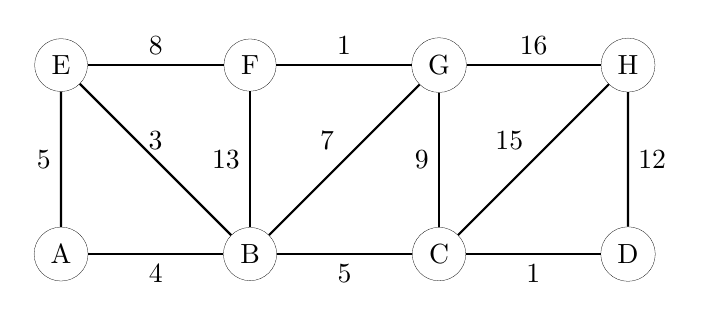
\begin{tikzpicture}
        [thick,scale=0.8, every node/.style={scale=1}]
        %		\node[circle] (n0){A};
        \node[circle, draw, line width=0.1pt] (a) at (-4.5,0){A};
        \node[circle, draw, line width=0.1pt] (b) at (-1.5,0){B};
        \node[circle, draw, line width=0.1pt] (c) at (1.5,0){C};
        \node[circle, draw, line width=0.1pt] (d) at (4.5,0){D};
        \node[circle, draw, line width=0.1pt] (e) at (-4.5,3){E};
        \node[circle, draw, line width=0.1pt] (f) at (-1.5,3){F};
        \node[circle, draw, line width=0.1pt] (g) at (1.5,3){G};
        \node[circle, draw, line width=0.1pt] (h) at (4.5,3){H};
        \draw[-] (a) to node[below]{4} (b);
        \draw[-] (a) to node[left]{5} (e);
        \draw[-] (b) to node[below]{5} (c);
        \draw[-] (b) to node[above]{3} (e);
        \draw[-] (b) to node[left]{13} (f);
        \draw[-] (b) to node[above left]{7} (g);
        \draw[-] (c) to node[below]{1} (d);
        \draw[-] (c) to node[left]{9} (g);
        \draw[-] (c) to node[above left]{15} (h);
        \draw[-] (d) to node[right]{12} (h);
        \draw[-] (e) to node[above]{8} (f);
        \draw[-] (f) to node[above]{1} (g);
        \draw[-] (g) to node[above]{16} (h);
    \end{tikzpicture}
\end{figure}


\begin{table}[htbp]
    \begin{center}
        \begin{tabular}{|l|c|c|c|c|c|c|c|c|c| p{3cm}|}
            \hline
                        & vertex & \texttt{dis[A]} & \texttt{dis[B]} & \texttt{dis[C]} & \texttt{dis[D]} & \texttt{dis[E]} & \texttt{dis[F]} & \texttt{dis[G]} & \texttt{dis[H]} \\ \hline
            initial     & /      & 0               & $\infty$        & $\infty$        & $\infty$        & $\infty$        & $\infty$        & $\infty$        & $\infty$        \\ \hline

            iteration 1 & A      & 0               & 4               & $\infty$        & $\infty$        & 5               & $\infty$        & $\infty$        & $\infty$        \\ \hline
            iteration 2 & B      & 0               & 4               & 9               & $\infty$        & 5               & 17              & 11              & $\infty$        \\ \hline
            iteration 3 & E      & 0               & 4               & 9               & $\infty$        & 5               & 13              & 11              & $\infty$        \\ \hline
            iteration 4 & C      & 0               & 4               & 9               & 10              & 5               & 13              & 11              & 24              \\ \hline
            iteration 5 & D      & 0               & 4               & 9               & 10              & 5               & 13              & 11              & 24              \\ \hline
            iteration 6 & H      & 0               & 4               & 9               & 10              & 5               & 12              & 11              & 24              \\ \hline
            iteration 7 & G      & 0               & 4               & 9               & 10              & 5               & 12              & 11              & 24              \\ \hline
            iteration 8 & F      & 0               & 4               & 9               & 10              & 5               & 12              & 11              & 24              \\ \hline
        \end{tabular}
    \end{center}
\end{table}


\newpage

\titledquestion{Noise}[6]

The road of SC101 country is represented by an undirected graph $G = (V, E)$ and each vertex represents a city or an airport. The set of airports is represented by $T \subset V$.

A vertex $v$ is said to \textit{be effected by noise} from an airport $t$ if the length of the shortest path from $t$ to $v$ is not larger than $R$. We want to find all the vertices that have noise.

Please design an algorithm to solve this question. You may call any algorithm learned in lecture as a subroutine but be sure to indicate its input. You \textbf{don't} need to prove the correctness of your algorithm. Then, analyze your \textbf{time complexity}.

To get full credits, the time complexity of your algorithm should not exceed $O\left(\left(|V| + |E|\right) \log |V|\right)$.

\textbf{Input:}
\begin{itemize}
    \item $G = (V, E)$, where $V=\{1,2,\ldots, n\}$, $E=\{(u_i,v_i,w_i):i=1,2,\ldots, m\}$, $w_i > 0$
    \item $T = \{t_1, \ldots, t_{l}\}$, where $|T| = l$, $1 \le t_i \le n$
    \item A positive number $R$
\end{itemize}

\textbf{Output:} All vertices $v$ that are effected by noise from \textbf{at least one} airport $t \in T$.


\begin{solution} \\
    Use Dijkstra's algorithm to solve this problem.
    \begin{enumerate}
        \item Set the airports has the 0 distance and other cities has $\infty$ distance. Use adjacency list to restore the distance and use min-heap to choose which to visit.
        \item Pop the top element of the min-heap and traverse its neighbour, renew their distance if the new distance is lower than its past distance.
        \item Repeat the operations above until there is no vertex in the min-heap.
        \item Traverse the vertices set and output all vertices with distance less than R.
    \end{enumerate}
    Time complexity analysis: \\
    First we should build a min-heap of vertex with distance, which is O(VlogV), and traverse the set T to set the distance of airports to 0, which is O(V).
    Then for every vertex to be removed, we should find all his neighbour, thus the complexity will be O(E) $\cdot$ O(logV).
    So that the whole time complexity is O(VlogV+ElogV).
\end{solution}






\newpage

\titledquestion{Travel}[8]

There is a country with $n$ cities and $m$ directed edges. The edge from $u$ to $v$ has a length $w_{u,v}$.
Traveler Bob is starting at city $1$ and going to city $n$.

Bob can either take \emph{car} or \emph{train} as his vehicle.
Suppose Bob is now at city $v_0$, and there is a path $v_0\rightarrow v_1\rightarrow \cdots \rightarrow v_k$.
Then he can go to $v_k$ through this path, either by car with a cost $\sum_{i=1}^k w_{v_{i-1}, v_i}$ (the sum of the weights of the edges in this path), or by train with a cost $t_{v_0} + c\times k$, where $t_{v_0}$ is the price of train ticket at city $v_0$, $c$ is a constant, and $k$ is the number of edges in this path.

Bob can freely decide which vehicle to take at any city. He can switch his vehicle multiple times. His goal is to minimize the total cost.

Please design an algorithm to solve this question. You may call any algorithm learned in lecture as a subroutine but be sure to indicate its input. You \textbf{don't} need to prove the correctness of your algorithm. Then, write your \textbf{time complexity}.

To get full credits, the time complexity of your algorithm should not exceed $O\left(\left(n + m\right) \log n\right)$.

\textbf{Input. } $n$, $m$, $E=\{(u_i,v_i,w_{u_i,v_i}>0):i=1,2,\ldots, m\}$, $\{t_i\}_{i=1}^n>0$, $c>0$.

\textbf{Output. } The minimal total cost.

\begin{solution} \\
    We can regard the station as a new city which shares the same location with this city.
    We can go to the station from city at the cost of $t_v$, and also can go to the city from station with no cost.
    Of course, we cannot go to the station and then go back to the city. First go to city then go back to station is also not allowed.
    Thus we copy graph G and get a new station graph G' with every edges' weight is c, and every vertex in G has an edge with weight $t_v$ to g' and 0 in opposite.
    Then use Dijkstra's algorithm to traverse all the vertices in G and G', with the number of vertices being 2n and number of edges being 2m+2n.
    The time complexity is O((2n+2m+2n)log(2n)) = O((m+n)logn).
\end{solution}







\end{questions}

\end{document}